%Chapter 7

\chapter{Simulation and Analysis} % Write in your own chapter title
\label{ch:Plasticity Model}
\lhead{Simulation and Analysis} % Write in your own chapter title to set the page header

In this chapter the ability of the Lemaitre damage model and it's variants to accurately predict fracture in wire drawing processes is assessed. The phase field fracture model is unsuitable for investigating this behaviour as it requires a very fine mesh making it computationally expensive. Another issue with it is that the existing phase field fracture models would require further developments to better account for crack-closure effects. Such a development is beyond the scope of this work. 

\section{Setup}

For each simulation, wire flows into the inlet patch, with the simulation being
carried out until consistent values are reached along the wire for its properties after exiting the die outlet. The wire is continuously being pulled in the axial direction by a fixed increment of displacement at each time step.

\begin{table}[htb]
	\centering
		\begin{tabular}{cccc} \hline
		    %Loading Conditions \\ \hline 
		    Applied Total Displacement & $u$ & $300\ mm$ \\
		    Uncoupled Displacement & $u$ & $50\ mm$ \\
		    Time Step & $\Delta t$ & $0.001\ s$ \\
			Displacement Increment  & $\Delta u$ & $2\ mm$   \\
			Friction Coefficient & $\mu$ & $0.1$ \\
			\hline
		\end{tabular}
	\caption{Loading conditions for wire drawing case}
	\label{tab:material_properties}
\end{table}

\begin{table}[htb]
	\centering
		\begin{tabular}{cccc} \hline
		    %Loading Conditions \\ \hline 
		    Die Inlet Diameter & $16\ mm$ \\
		    Die Outlet Diameter & $11.6276\ mm$ \\
		    Die Outer Diameter & $20\ mm$ \\
		    Die Angle & $20^{\circ}$ \\
		    Wire Length & $300\ mm$ \\
		    Wire Diameter & $13\ mm$ \\
			\hline
		\end{tabular}
	\caption{Die and wire geometry}
	\label{tab:material_properties}
\end{table}

For these wire drawing cases, an initial contact is applied so that at the first time step the simulation is as shown in figure. This can lead to localisation's of plastic strain in the region of the wire in contact with the die. As the simulation moves forward however, a more settled solution is obtained. 


\begin{figure}[t!]
	\centering
		\subfigure[Initial contact at first time step] {\label{airbus}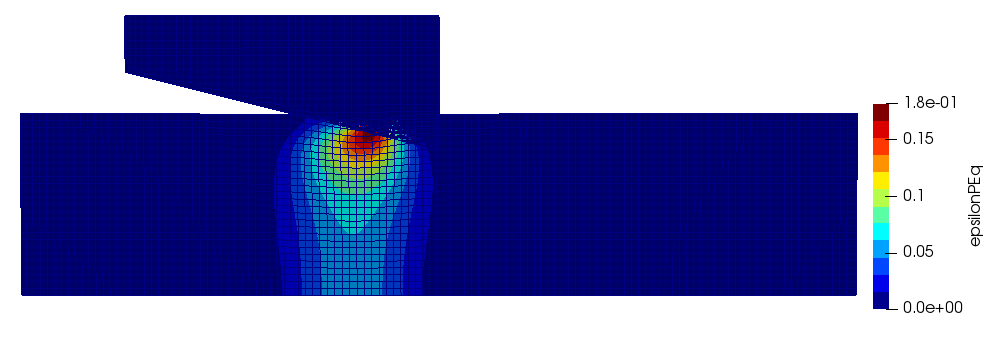
\includegraphics[width=0.8\textwidth]{./Figures/SimulationAndAnalysis/initialContact.png}}		
	  \qquad
		\subfigure[Equivalent plastic strain after $160mm$ displacement] {\label{boeing} 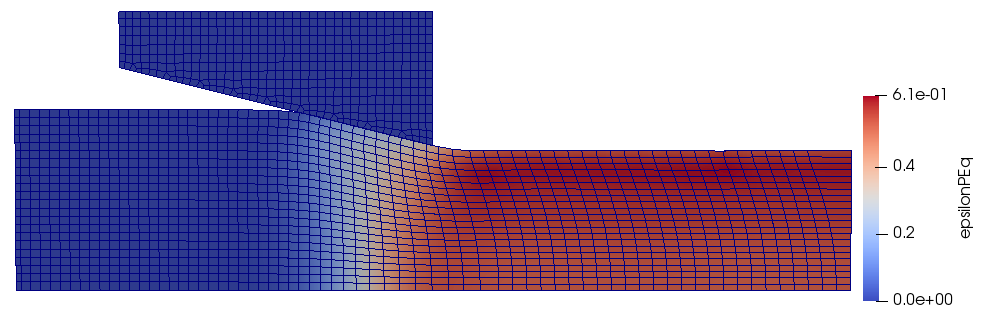
\includegraphics[width=0.8\textwidth]{./Figures/SimulationAndAnalysis/settledEquivalentPlasticStrain.png}}
        \qquad
  	\subfigure[Damage after $160mm$ displacement] {\label{boeing} 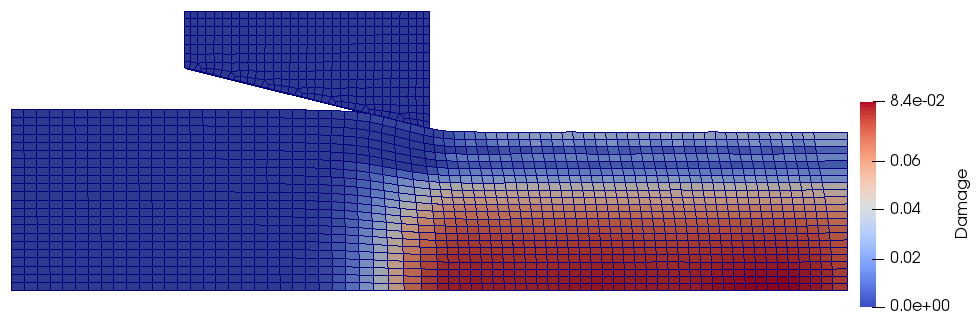
\includegraphics[width=0.8\textwidth]{./Figures/SimulationAndAnalysis/consistentDamageProfile.png}}
		
		\caption{Wire drawing simulation}
	\label{label_for_entire_figure}
\end{figure}
\FloatBarrier

\textbf{Incorporating Damage}

This set-up can lead to issues when incorporated damage however, particularly in cases with large reductions and high die angles. The high amount of deformation in this region can often lead to a large amount of damage accruing and an unstable numerical solution. It was found that this issue can be ameliorated by setting the damage to only begin evolving in the wire after the wire has already gone a user defined displacement.

\begin{figure}[htb]
\begin{center}
	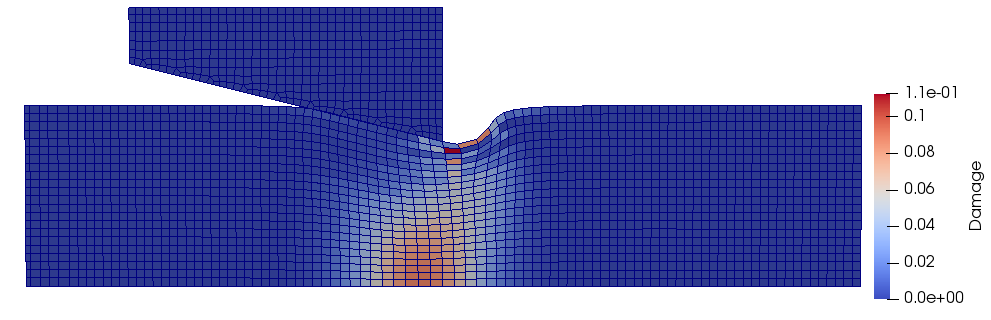
\includegraphics[width=0.7\textwidth]{./Figures/SimulationAndAnalysis/issueWithDamage.png}
\caption{Issue with incorporating damage at initial stages of case}
\label{fig:notchedRoundBAr}
\end{center}
\end{figure}